% !TeX root = ../main.tex
\section{Описание эксперимента}

\subsection{Выбор локации и времени наблюдения}

Для минимизации влияния многолучевого распространения радиоволн и затенения небесной полусферы высотными строениями в качестве площадки проведения эксперимента была выбрана открытая территория в районе станции метро «Котельники» (г.~Москва, координаты точки наблюдения: $55{,}6741^\circ\text{ с.ш.}$, $37{,}8582^\circ\text{ в.д.}$). В непосредственной близости от точки приёма в радиусе $50\text{ м}$ отсутствуют капитальные многоэтажные здания, что обеспечивает открытый обзор верхней полусферы небосвода. Положение выбранной локации на карте местности представлено на рисунке~\ref{fig:location}.

\begin{figure}[H]
    \centering
    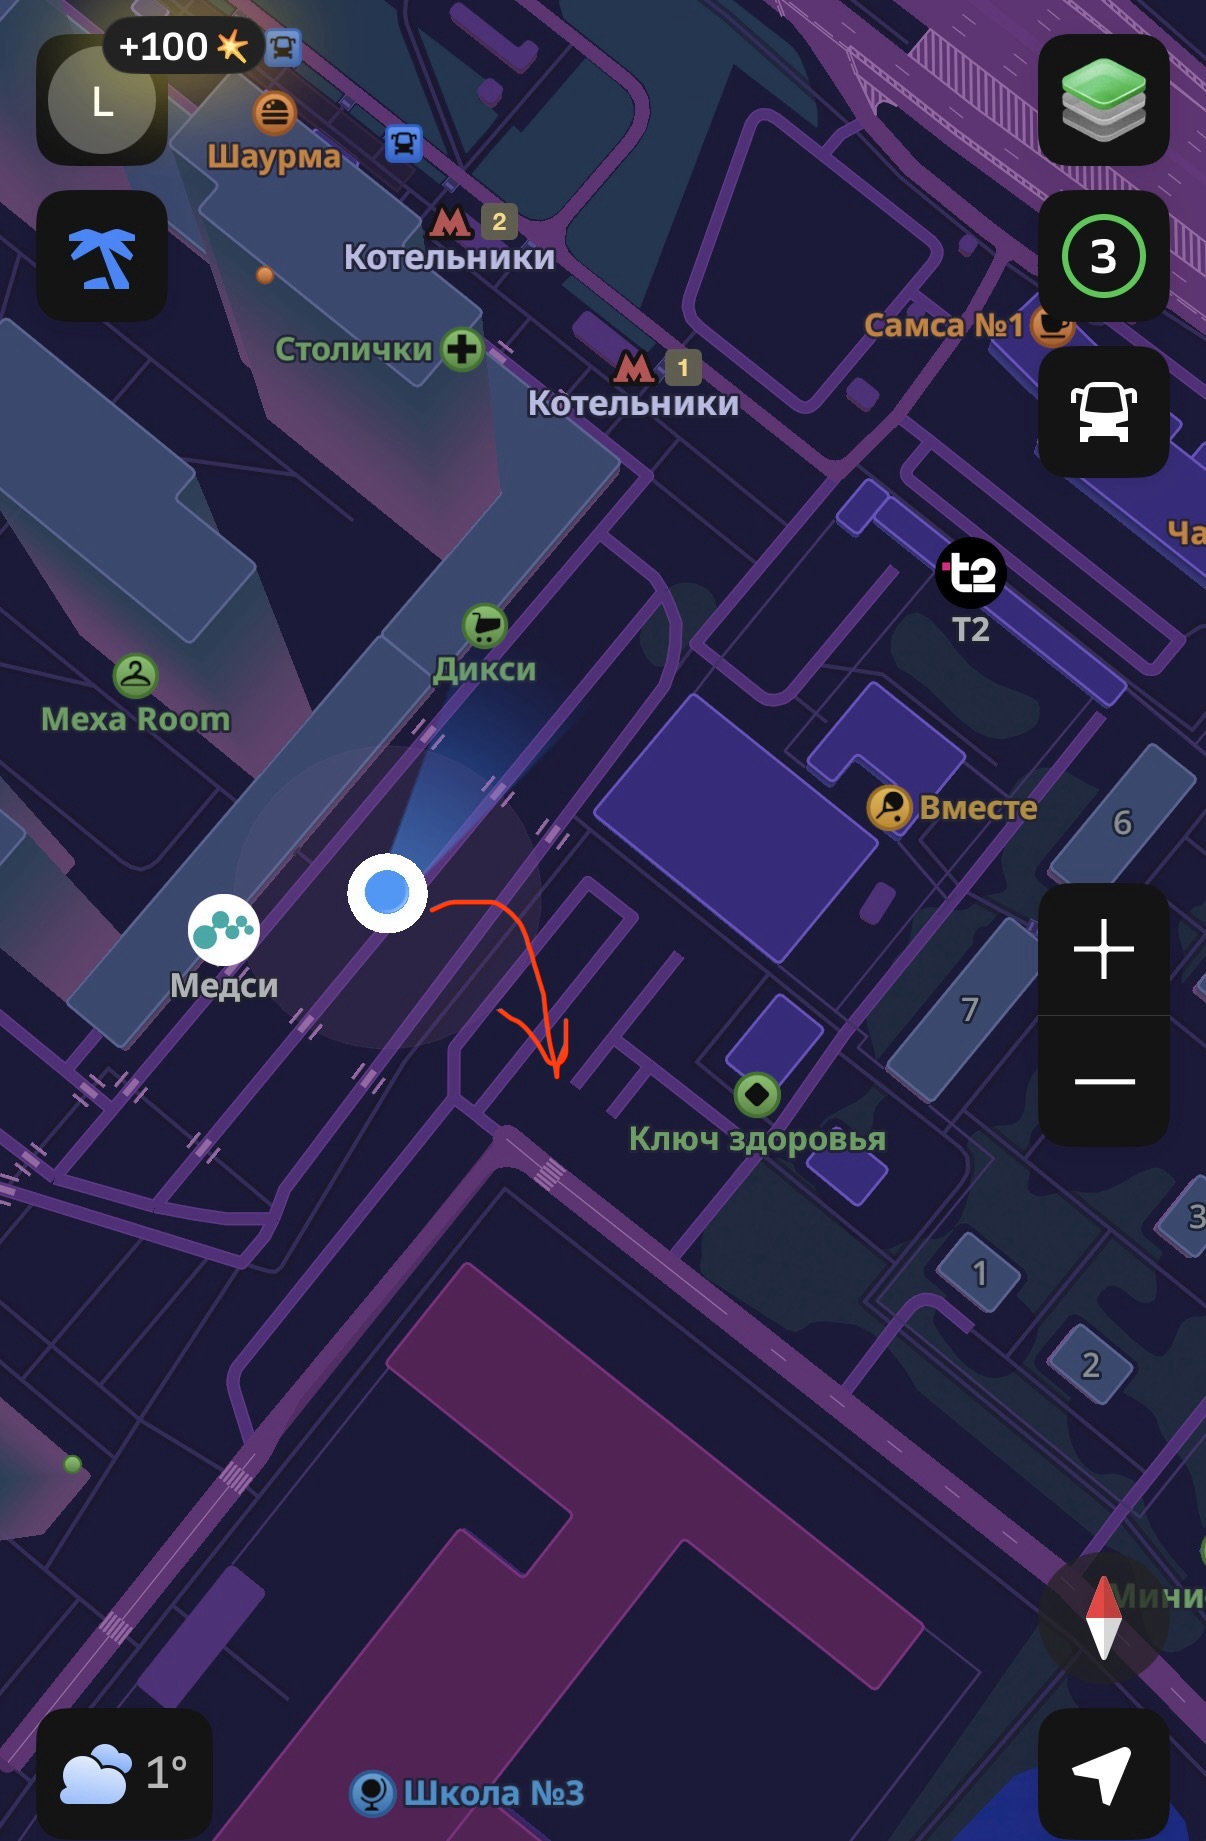
\includegraphics[width=0.55\textwidth]{IMG_4239.jpg}
    \caption{Расположение точки проведения эксперимента на карте местности}
    \label{fig:location}
\end{figure}

Наблюдения проводились 22~ноября 2026~года в $15{:}27$ по местному времени ($12{:}27\text{ UTC}$). Выбор момента фиксации был синхронизирован с предварительным расчётом эфемеридной обстановки таким образом, чтобы в зоне радиовидимости находилось максимальное количество навигационных космических аппаратов (НКА) основных глобальных созвездий.

\subsection{Аппаратное и программное обеспечение}

В связи с тем, что программный интерфейс ОС iOS ограничивает прямой доступ сторонних приложений к сырым измерениям отношения несущей к спектральной плотности шума ($C/N_0$), эксперимент проводился с использованием двух устройств в одной точке наблюдения. На основном смартфоне Apple~iPhone с помощью специализированного приложения GNSS~View осуществлялись построение карты небосвода (SkyView), контроль геометрических факторов точности (HDOP/VDOP) и фотофиксация положения космических аппаратов в режиме дополненной реальности (AR). Параллельно для регистрации численных значений $C/N_0$ по каждому сопровождаемому спутнику использовался контрольный смартфон Xiaomi~Redmi~A5 под управлением ОС Android (навигационный модуль на базе однокристальной системы Unisoc~T7250 с поддержкой систем GPS, ГЛОНАСС, Galileo и BeiDou) с установленным диагностическим пакетом GPSTest.

\subsection{Прогнозирование спутникового созвездия}

На предварительном этапе для заданных координат и времени наблюдения ($22.11.2026$, $15{:}27$ местного времени) была построена расчётная карта небосвода, приведённая на рисунке~\ref{fig:skyview_forecast}. Согласно расчётам геометрического фактора ухудшения точности, ожидаемая геометрия созвездия характеризуется значениями $HDOP = 0{,}32$ и $VDOP = 0{,}51$, что соответствует высокой точности пространственного определения координат.

\begin{figure}[H]
    \centering
    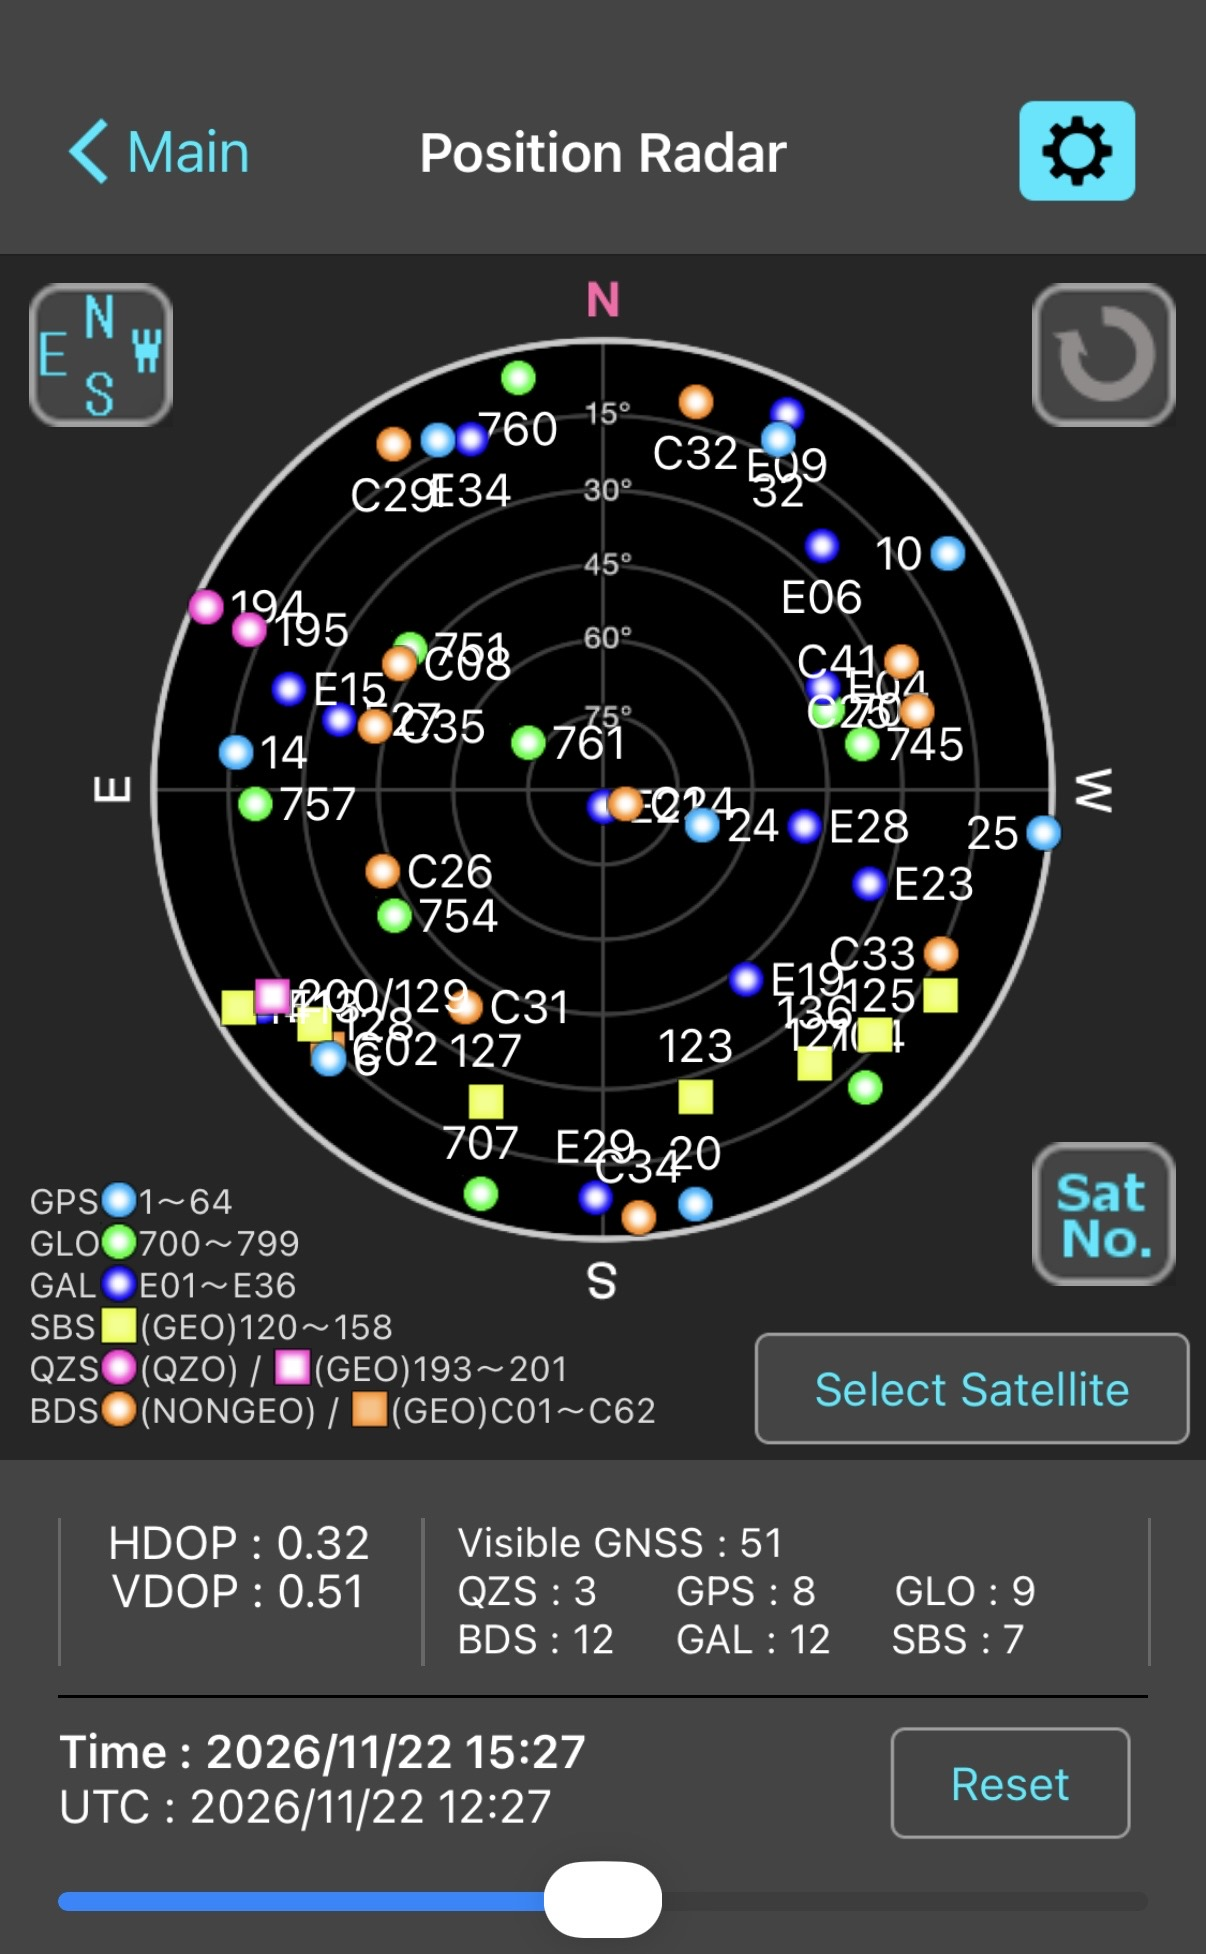
\includegraphics[width=0.55\textwidth]{IMG_4240.jpg}
    \caption{Расчётная карта небосвода (SkyView) на момент времени $15{:}27$ ($12{:}27\text{ UTC}$)}
    \label{fig:skyview_forecast}
\end{figure}

Всего в зоне радиовидимости над горизонтом в заданный момент времени прогнозируется $51$ космический аппарат, включая $41$ НКА четырёх основных глобальных систем (GPS, ГЛОНАСС, Galileo, BeiDou). Сводные данные о количестве и номерах ожидаемых спутников основных ГНСС систематизированы в таблице~\ref{tab:forecast}.

\begin{table}[H]
    \centering
    \caption{Прогнозируемый состав рабочего созвездия на $15{:}27$ ($12{:}27\text{ UTC}$)}
    \label{tab:forecast}
    \begin{tabular}{|l|c|p{9.5cm}|}
        \hline
        \textbf{Система ГНСС} & \textbf{Кол-во} & \textbf{Номера ожидаемых спутников (PRN / системный номер)} \\
        \hline
        GPS (США) & 8 & 01, 10, 14, 21, 24, 25, 28, 32 \\
        \hline
        ГЛОНАСС (Россия) & 9 & 707, 735, 745, 754, 757, 760, 761, 762, 765 \\
        \hline
        Galileo (ЕС) & 12 & E04, E06, E09, E13, E15, E19, E21, E23, E24, E28, E34, E36 \\
        \hline
        BeiDou (Китай) & 12 & C02, C08, C25, C26, C29, C31, C32, C33, C35, C38, C41, C45 \\
        \hline
    \end{tabular}
\end{table}

\subsection{Методика проведения натурных наблюдений}

Прибыв на выбранную локацию к назначенному времени, экспериментатор запустил приложение GNSS~View. Для гарантированного завершения процессов холодного и тёплого старта, загрузки актуального альманаха, эфемерид и стабилизации координатного решения приёмник выдерживался на месте неподвижно в течение $4\text{ минут}$. По истечении времени стабилизации в $15{:}27$ была выполнена фотофиксация небесной полусферы с наложением расчётного положения спутников в режиме дополненной реальности в двух секторах обзора.

\begin{figure}[H]
    \centering
    \begin{minipage}[b]{0.48\textwidth}
        \centering
        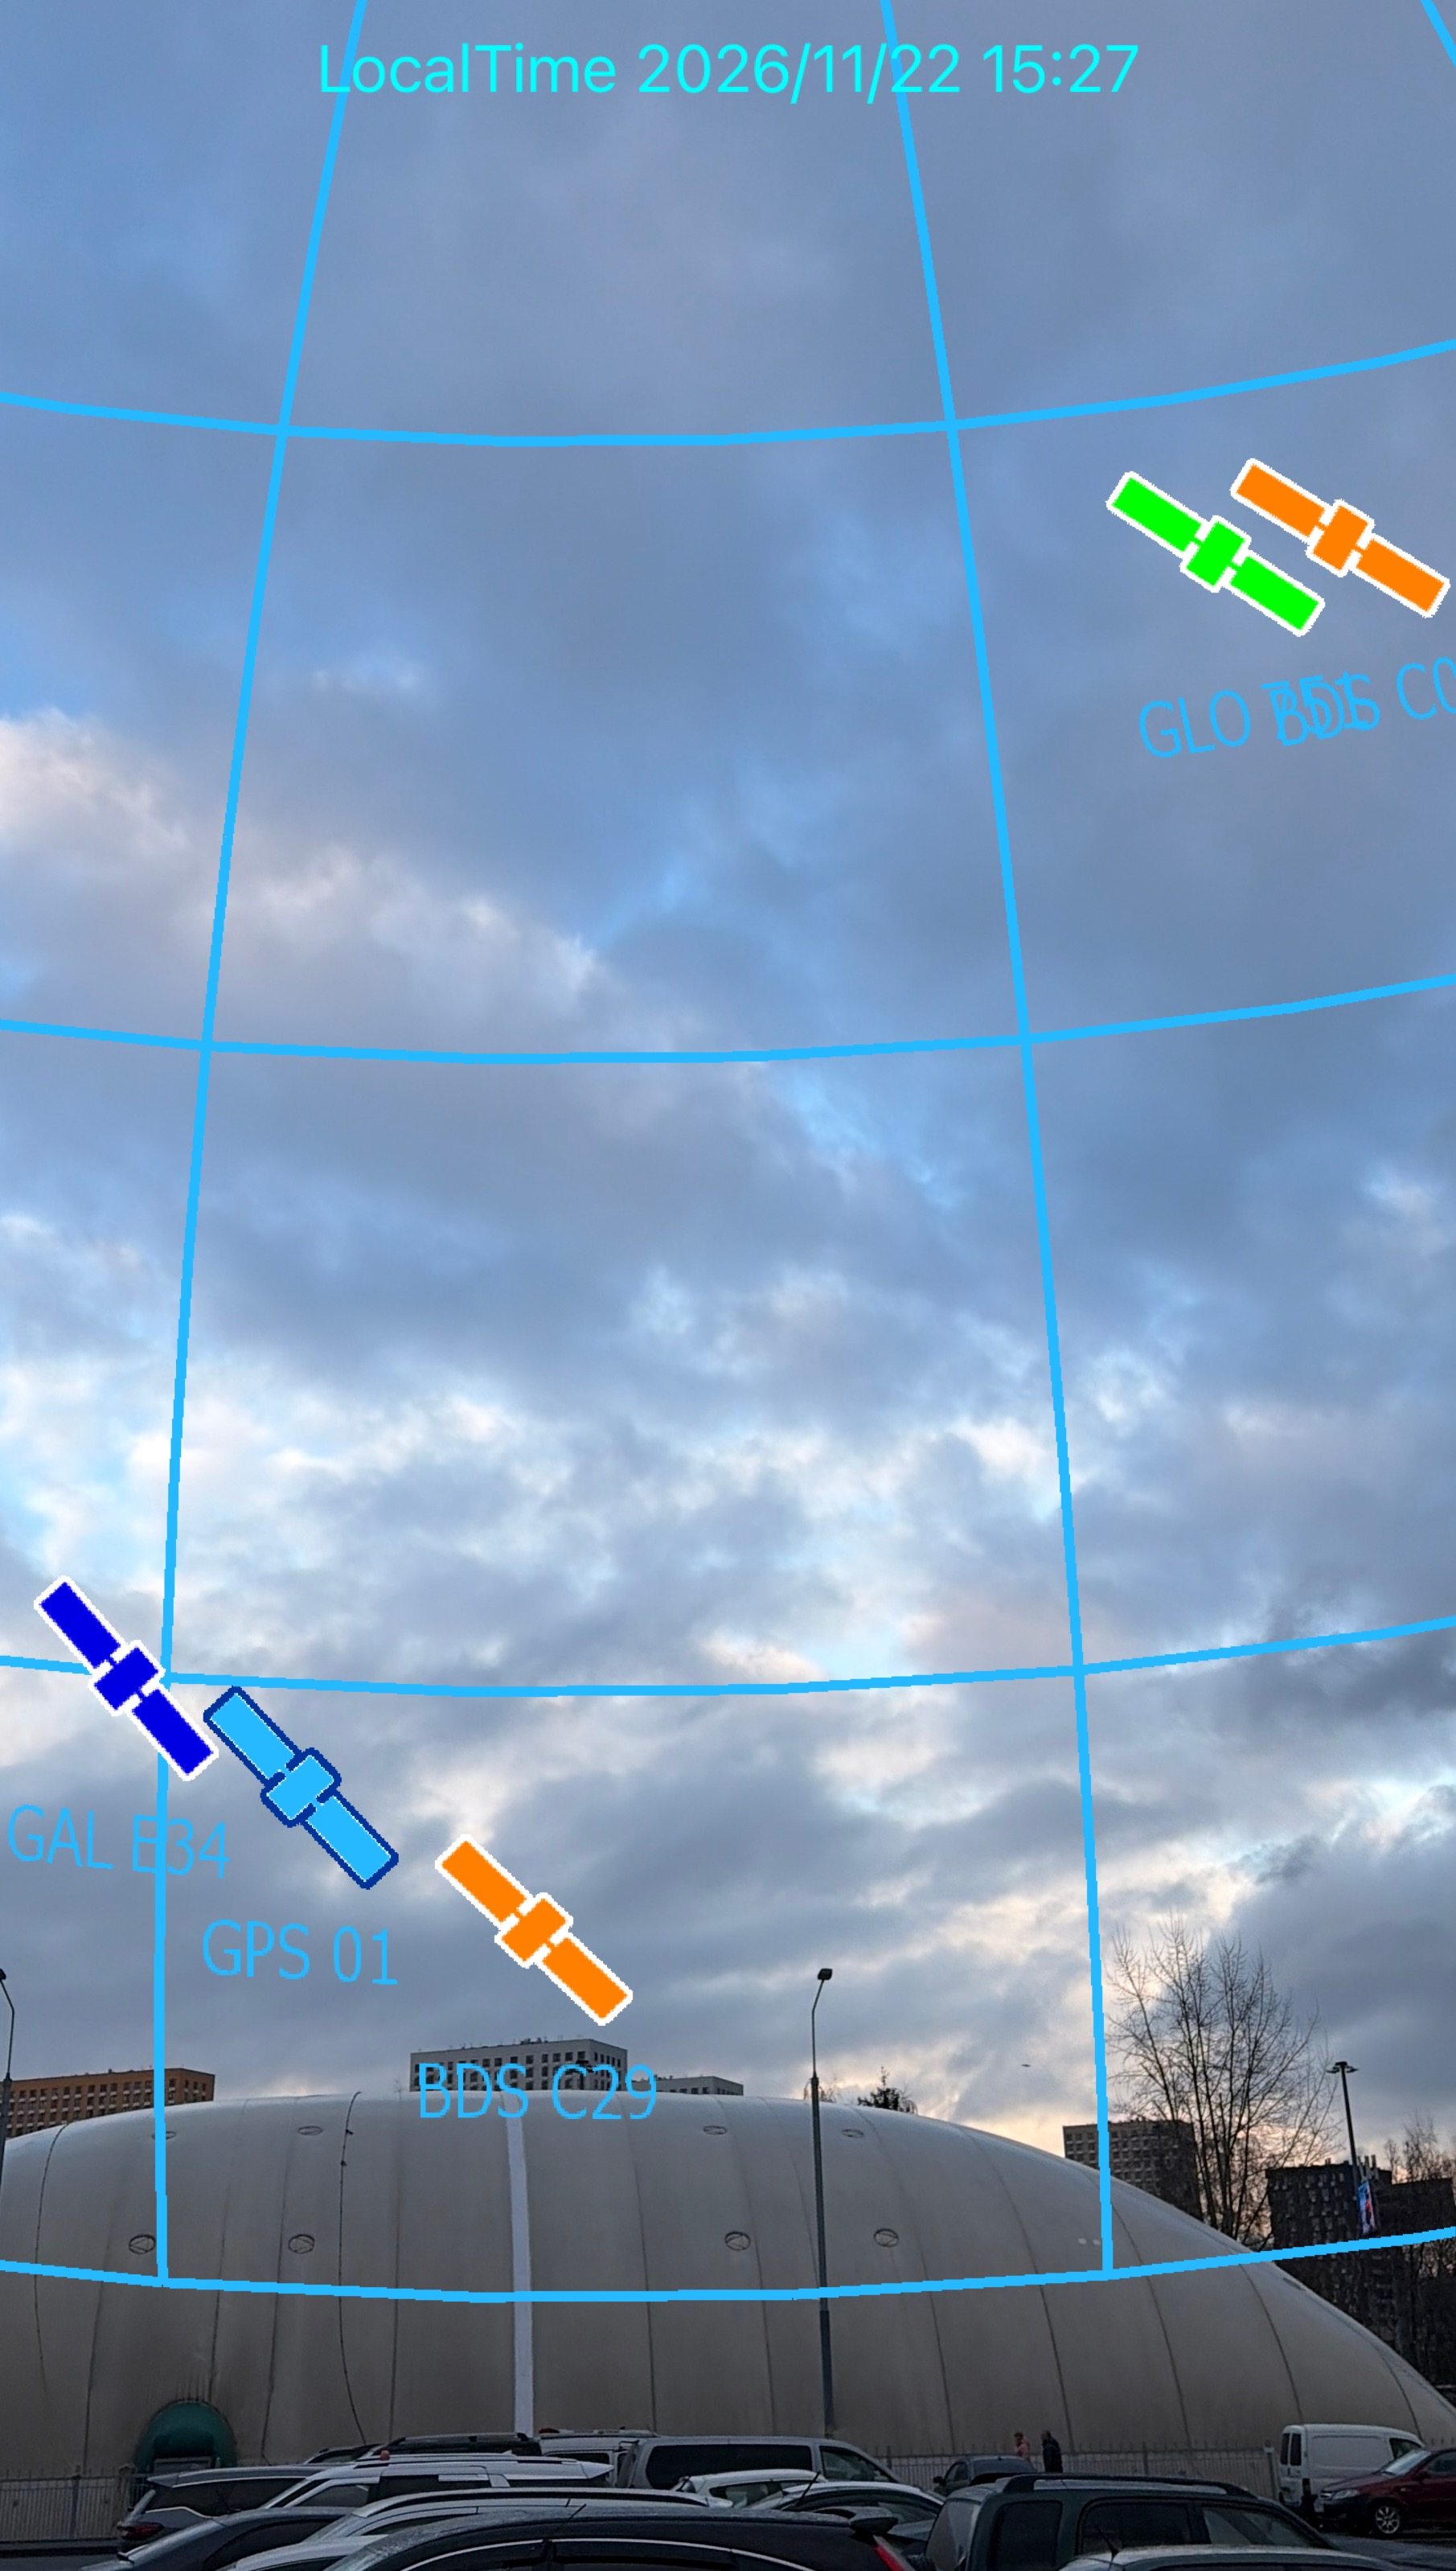
\includegraphics[width=\textwidth]{IMG_4241.jpg}
        \caption{AR-визуализация НКА (сектор 1)}
        \label{fig:ar_skyview_1}
    \end{minipage}
    \hfill
    \begin{minipage}[b]{0.48\textwidth}
        \centering
        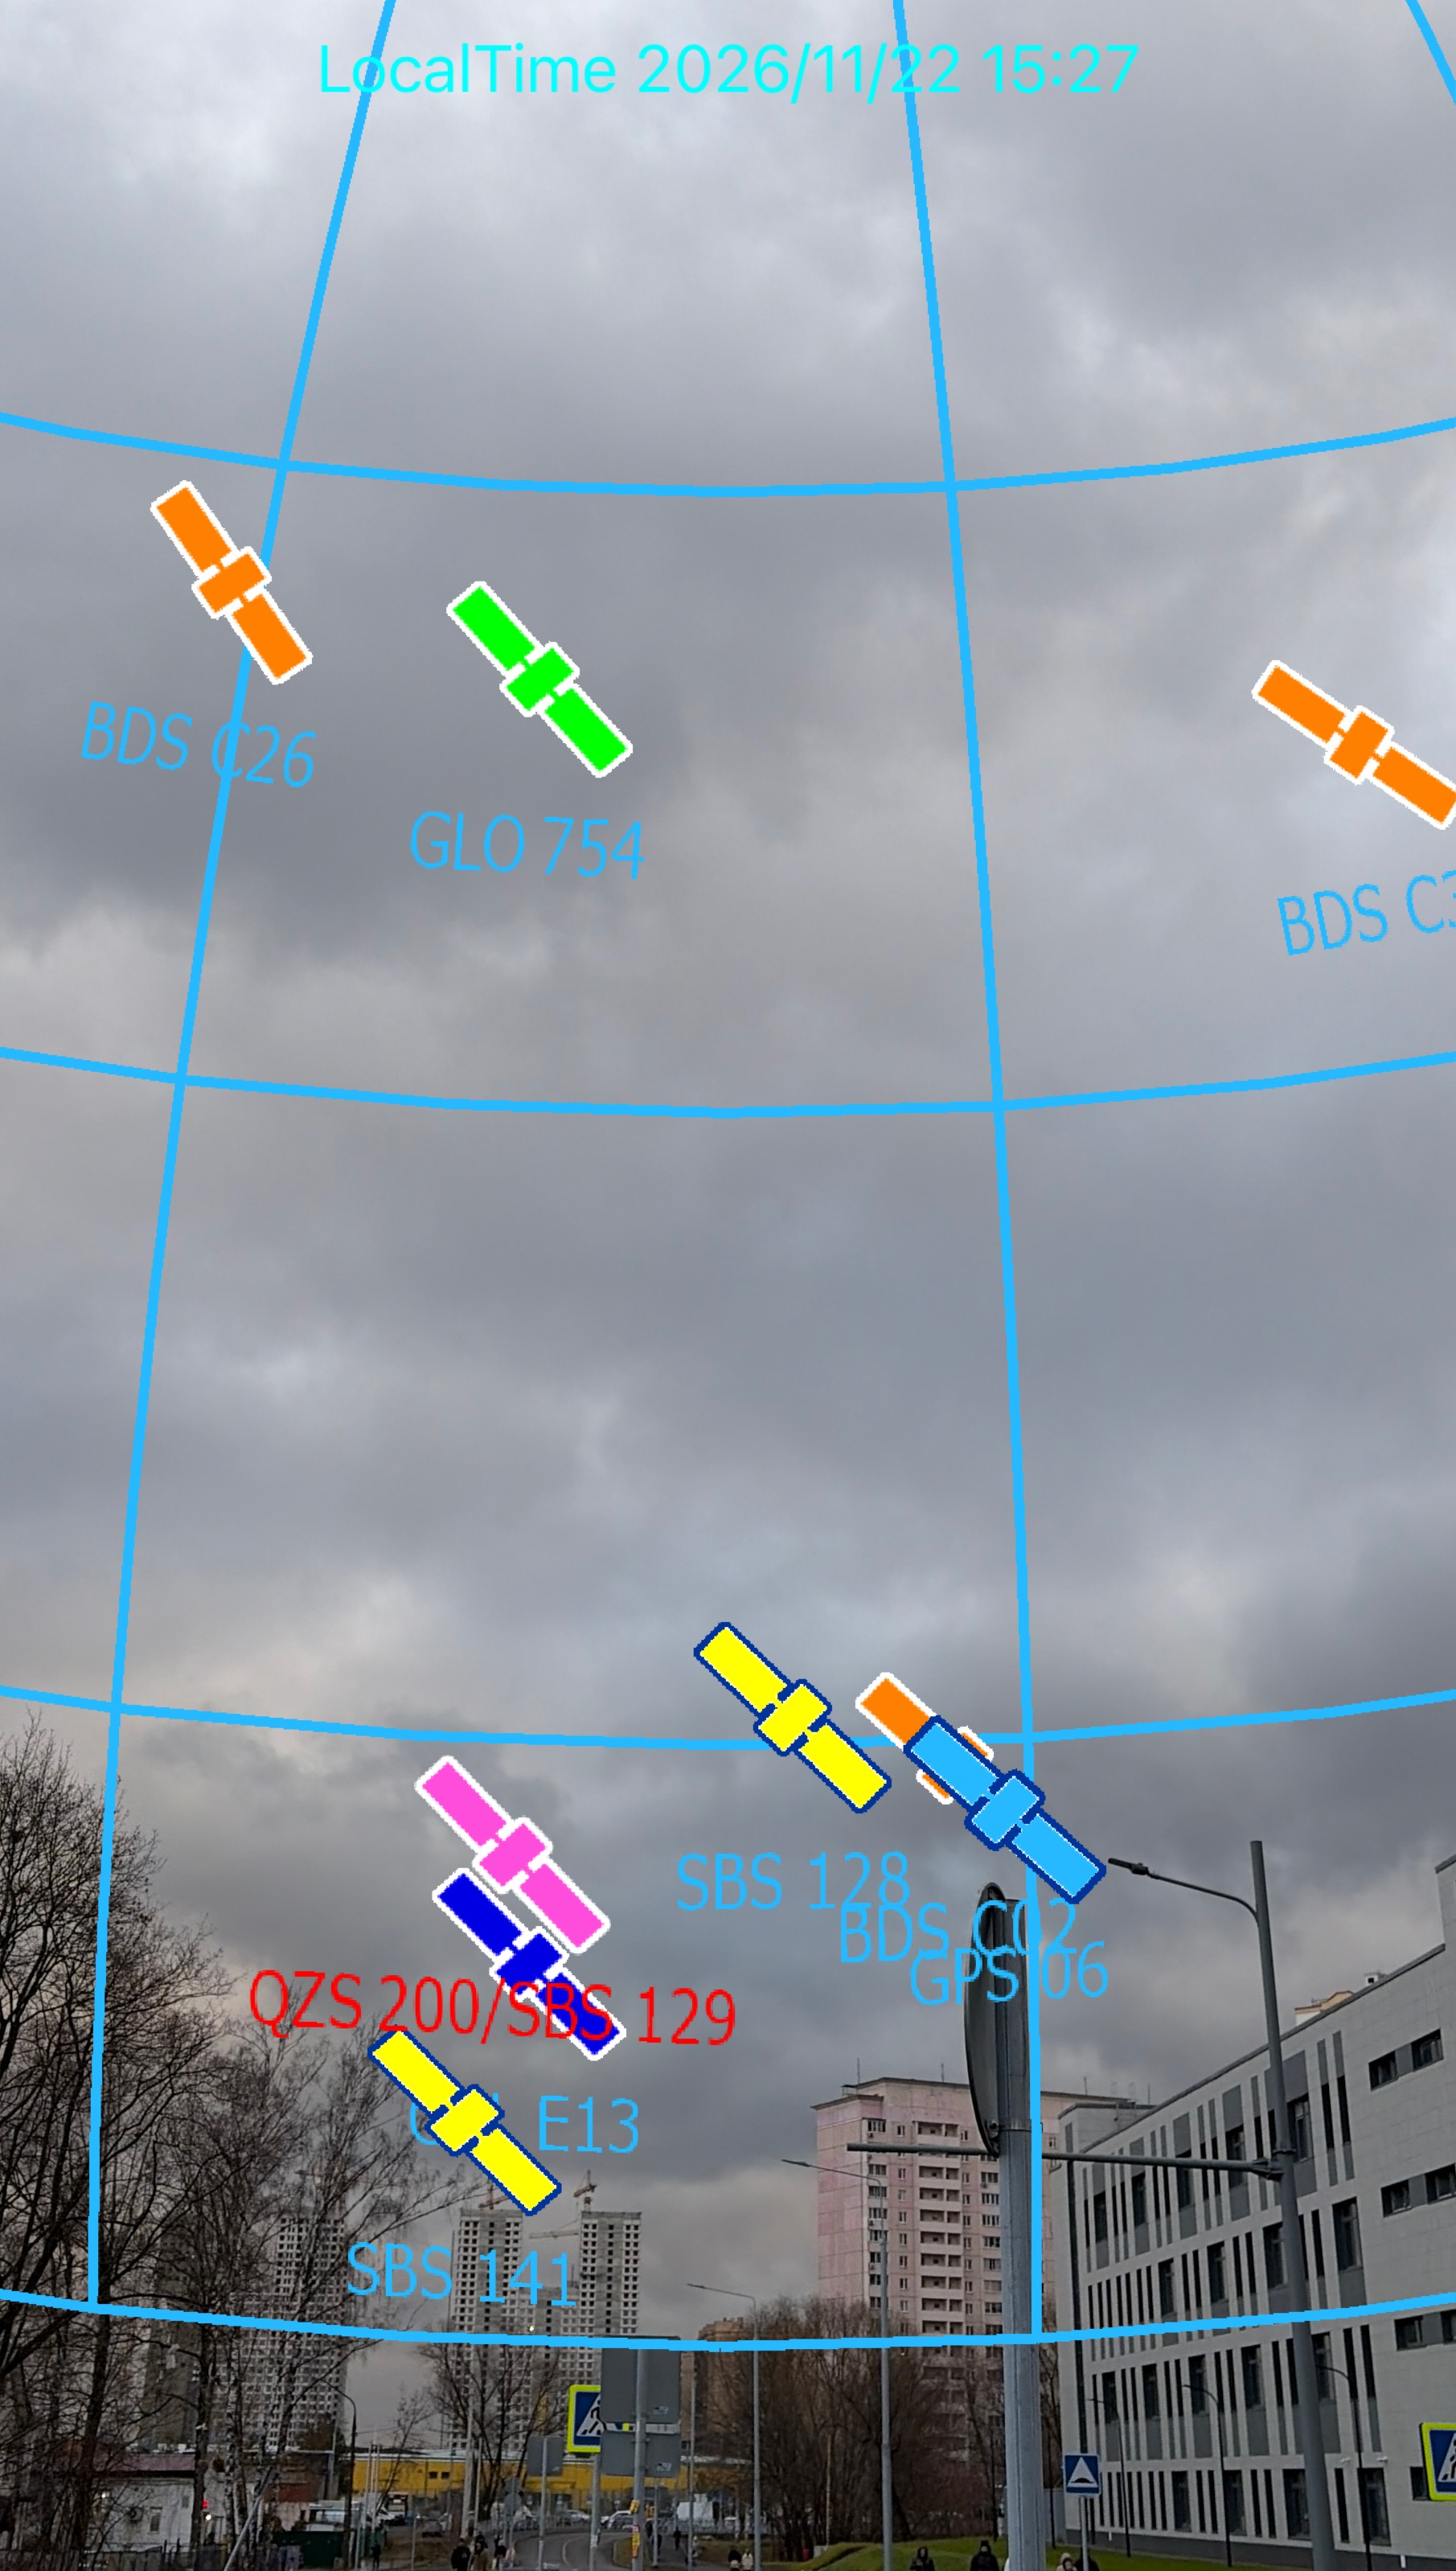
\includegraphics[width=\textwidth]{IMG_4242.jpg}
        \caption{AR-визуализация НКА (сектор 2)}
        \label{fig:ar_skyview_2}
    \end{minipage}
    \label{fig:ar_skyview}
\end{figure}
